\documentclass{beamer}
%%%%%% UNOFFICIAL ICL BEAMER TEMPLATE V.0.1 %%%%%%
% This is a basic LaTeX Beamer template that I customised to have the logo of ICL and a background picture. Mind that this is NOT an official ICL template but it may still be useful for informal presentations.
% The official ICL graphical identity resources can be found here: http://www3.imperial.ac.uk/graphicidentity
% Please drop me an e-mail or comment via Twitter @AJunyentFerre if you found this was useful or have any suggestion to improve it.
%%%%%%

\usepackage[english]{babel}

%%%%%% THE FOLLOWING FILE CONTAINS THE STYLE DEFINITIONS %%%%%%
\input{header.tex}
%%%%%%

%%%%%% TITLE, AUTHOR, DATE DEFINITIONS %%%%%%
\title{Agent Foundations}
\author{Daniel C}
\date{19th April 2026}
%%%%%%

\begin{document}






\frame{\titlepage}\section{Introduction}



\frame{\frametitle{Why Agent Foundations?}
	\begin{block}{Aligning a system that doesn't exist yet}
		{\tiny
		\begin{itemize}
			\item We are trying to align a superintelligence that does not yet exist, under conditions unlike anything we have observed
			\item Agent foundations studies the properties of intelligent agents \textit{in general}, rather than any specific instantiation -- so that we can reason about the behavior of superintelligent agents in advance
            \item We need to get alignment right on the \textit{first critical try} when operating at a dangerous level of intelligence -- unaligned operation at that level may be catastrophic, and we do not get to iterate. We cannot rely on trial-and-error the way science usually does
			\item Even if we try to learn about superintelligent agents empirically from weaker systems, we still need a theory of \textit{what kinds of} properties generalize to greater intelligence -- and that is itself a theory in agent foundations		\end{itemize}
		}
	\end{block}
}



\section{Reflective Stability}
\frame{\frametitle{Reflective Stability}
	\begin{block}{Self-modification and the stability of goals}
		{\tiny
		\begin{itemize}
			\item A superintelligence will be capable of: rewriting its own source code, building a smarter successor AI, and radically revising its world model (e.g.\ learning new physics, ontology shifts)
			\item A property is \textit{reflectively stable} if it remains invariant under all such self-modifications
			\item Any safety guardrail we instill is irrelevant if the AI can self-modify to remove it, or build a successor that lacks it
			\item For a sufficiently capable goal-directed agent, \textbf{nothing sticks around unless it has to} -- every property, architecture, constraint, and conceptual scheme is subject to being optimized away
			\item To guarantee a property persists (e.g.\ ``this machine doesn't kill all humans''), we must understand what kinds of things \textit{can} stick around under this pressure -- most things don't
			\item Reflectively stable properties do \textbf{not} self-correct: if Gandhi doesn't want to kill people, he will refuse a pill that makes him want to kill people
            \item Contrast with properties that \textit{do} self-correct: a false belief about the world (e.g.\ a mistaken belief about gravity) will be corrected as the AI gets smarter
		\end{itemize}
		}
	\end{block}
}


\frame{\frametitle{Goodhart's Law and Robust Concepts}
	\begin{block}{When proxy measures break under optimization}
		{\tiny
		\begin{itemize}
			\item Let $V$ be the true goal, $U$ a proxy observed to correlate with $V$, and $X$ the gap between them: $U = V + X$
			\item A point with large $U$ will likely have large $V$ -- but also large $X$; so optimizing $U$ selects not just for $V$ but also for the discrepancy between $U$ and $V$
			\item The harder you optimize, the more $V$ lags behind $U$
			\item This is already a problem with weak optimization; whereas a superintelligence will impose extreme optimization pressure to the proxy
            \item Aligning a superintelligence requires us to have robust concepts or "True names" that don't break down even when they are subjected to extreme optimization pressure
		\end{itemize}
		}
	\end{block}
    \begin{block}{Examples of "True names" we may want}
		{\tiny
		\begin{itemize}
			\item \textbf{Optimization}
			\item \textbf{Goals} 
			\item \textbf{World models}
            \item \textbf{Embeddedness}
		\end{itemize}
		}
	\end{block}
}

\section{Coherence}
\frame{\frametitle{Reasoning About Ideal Intelligence}
	\begin{block}{Coherence and dominated strategies}
		{\tiny
		\begin{itemize}
			\item An agent with circular preferences (A $\succ$ B $\succ$ C $\succ$ A) can be \textit{money-pumped}: an adversary cycles them through trades, extracting a small fee each round, leaving the agent strictly worse off after every cycle
			\item \textbf{Dutch book setup:} formalize an agent's degrees of belief as \textit{betting prices} -- for each event $X$, the agent posts a price $p \in [0,1]$, meaning they are willing to buy or sell a contract that pays \$1 if $X$ turns out to be true and \$0 otherwise, at price $p$
			\item The agent's price $p$ for $X$ thus represents their subjective probability that $X$ is true
			\item A Dutch book is a combination of such contracts, bought or sold at the agent's own posted prices, that guarantees the agent a net loss regardless of how the world turns out
			\item An agent whose prices violate the probability axioms executes a \textit{dominated strategy} -- a Dutch book can always be constructed against them, and they can be exploited indefinitely
			\item \textbf{Key result:} an agent is immune to Dutch books if and only if their betting prices satisfy the axioms of probability -- Bayesianism and Expected utility maximization falls out of the requirement to avoid dominated strategies
            \item \textbf{Sidenote:} Measuring stick of utility problem
		\end{itemize}
		}
	\end{block}
    
}


\frame{\frametitle{Dualistic agents}
	\begin{block}{Dualistic agents}
		{\tiny
		\begin{itemize}
			\item This is Alexei, and Alexei is playing a video game.
    \begin{figure}
        \centering
        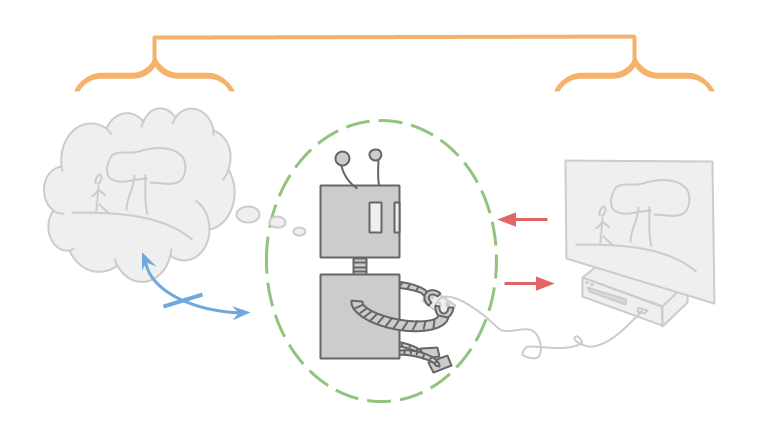
\includegraphics[width=0.3\linewidth]{ekude8k13w2p8nm8mhfc.png}
        
        \label{fig:placeholder}
    \end{figure}
        \item Clear input \& output channel
        \item Can hold the entire video game inside his mind
        \item Does not have to think about himself, only optimizing the environment
        \item Standard models of agency (e.g. EU maximization, AIXI) usually operate under this dualistic picture
    
		\end{itemize}
		}
	\end{block}
    
}

\section{Embedded agents}
\frame{\frametitle{Embedded agents}
	\begin{block}{Embedded agents}
		{\tiny
		\begin{itemize}
			\item This is Emmy. Emmy is playing real life. 
    \begin{figure}
        \centering
        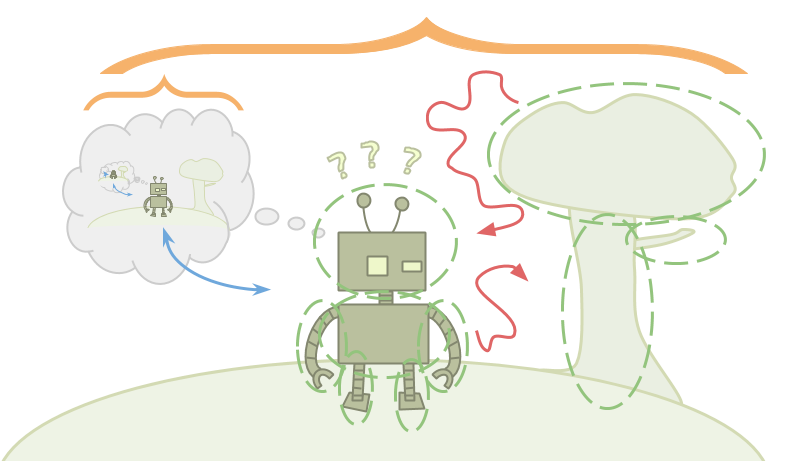
\includegraphics[width=0.3\linewidth]{quqsoo5xeq4clo0wzjcf.png}
        
        \label{fig:placeholder}
    \end{figure}
        \item The environment contains her, Emmy is just one part of the environment
        \item No well defined input \& output channel
        \item Cannot hold the environment inside her own head
        \item Environment may contain copies of her
        \item Emmy is made out of the same pieces that the rest of the environment is made out of
        \item Since Emmy is within the environment that she is manipulating, she is also going to be capable of self-improvement
        \item We would like a theory of consequentialist agency that is consistent with this embeddedness setting
    
		\end{itemize}
		}
	\end{block}
    
}



\frame{\frametitle{Self-Modification and Vingean Reflection}
	\begin{block}{Tiling agents: designing a successor}
		{\tiny
		\begin{itemize}
			\item A sufficiently intelligent agent $A_1$ may choose to build a successor agent $A_0$ (or equivalently, rewrite its own source code -- self-improvement is a special case of constructing a successor)
			\item \textbf{Vingean uncertainty:} $A_1$ cannot predict the exact decisions of something as smart or smarter than itself -- if it could, it would be just as smart. 
			\item So $A_1$ cannot verify $A_0$'s safety by simulating it step by step. Instead, $A_1$ must reason \textit{abstractly} about properties of $A_0$'s design, guaranteeing that whatever $A_0$ does falls within acceptable bounds. Just as Deep Blue's designers could reason that the program was ``trying to win'' without knowing its exact moves
            \item In addition, $A_1$ cannot anticipate all future observations that $A_0$ will receive
			\item \textbf{Tiling:} we want $A_1$ to be able to approve the construction of successors that is similar to itself (e.g.\ same software, different hardware)

		\end{itemize}
		}
	\end{block}
	
}

\frame{\frametitle{Self-Modification and Vingean Reflection}
	\begin{block}{How can $A_1$ trust $A_0$?}
		{\tiny
		\begin{itemize}
			\item $A_1$ and $A_0$ share a satisficing goal $\mathcal{G}$. $A_0$ only takes actions it can \textit{prove} achieve $\mathcal{G}$
			\item $A_1$ inspects $A_0$'s source code and verifies: if $A_0$ is constructed, then any action $A_0$ takes was proved (in $A_0$'s proof system) to achieve $\mathcal{G}$:
			$$A^1 \Vdash \bar{A}^0 \to (\forall b_i \in \textit{Acts}^0 : \bar{b}_i \to \Box_0[\bar{b}_i \to \mathcal{G}])  \qquad (2.3)$$
			{\scriptsize ($\bar{A}^0$ = ``$A_0$ is constructed'', \; $\Box_0[\phi]$ = ``there exists a proof of $\phi$ from $A_0$'s axioms'')}
			\item But this only tells $A_1$ that $A_0$ \textit{acts on what $A_0$'s proof system certifies} -- not that what $A_0$'s proof system certifies is actually \textit{true}
			\item To close this gap, $A_1$ needs to trust $A_0$'s proof system: whenever $A_0$ proves something, it is actually true
			$$A^1 \Vdash \forall b_i : (\Box_0[\bar{b}_i \to \mathcal{G}] \to (\bar{b}_i \to \mathcal{G})) \qquad (2.4)$$
			\item Combining (2.3) and (2.4): $\quad A^1 \Vdash \bar{A}^0 \to (\forall b_i \in \textit{Acts}^0 : (\bar{b}_i \to \mathcal{G}))$
			\\ {\scriptsize ``If $A_0$ is constructed, then any action $A_0$ takes achieves the goal''}
		\end{itemize}
		}
	\end{block}
}


\frame{\frametitle{The Löbian Obstacle}
	\begin{block}{The problem of self-trust}
		{\tiny
		\begin{itemize}
			\item When $A_1$ and $A_0$ use the \textit{same} proof system $L$, equation (2.4) becomes:
			$$L \vdash \forall \phi : (\Box \phi \to \phi)$$
			{\scriptsize ``Whenever $L$ can prove $\phi$, then $\phi$ is actually true'' -- $L$ vouches for its own proofs}
			\item This seems like a reasonable thing for a rational agent to believe: ``if I could prove $P$, then $P$ would be true''
			\item But \textbf{Löb's theorem} says: for any statement $C$, if $L \vdash \Box C \to C$, then $L \vdash C$
			\\ {\scriptsize The \textit{only} statements for which $L$ can assert ``if I could prove this, it would be true'' are statements $L$ could already prove anyway}
			\item Self-trust would imply that $L \vdash \Box(2+2=5) \to (2+2=5)$: ``if I could prove $2+2=5$, then $2+2=5$ would be true.'' But by Löb's theorem, this means $L \vdash 2+2=5$
			\item A consistent formal system cannot vouch for its own proofs in the abstract -- it can only trust a proof once it has \textit{witnessed it directly}
		\end{itemize}
		}
	\end{block}
	
}

\frame{\frametitle{The Löbian Obstacle}
		\begin{block}{Consequence for tiling agents}
		{\tiny
		\begin{itemize}
			\item $A_1$ can only trust $A_0$'s proofs if $A_0$ uses a \textit{strictly weaker} proof system than $A_1$
			\item Each successive agent in a chain of successor must use a weaker proof system than its predecessor -- a ``telomere'' of logical strength that shortens with each generation
			\item Eventually the chain runs out of trust, making indefinitely long chains of safe self-modification seemingly impossible
		\end{itemize}
		}
	\end{block}
	
}

\frame{\frametitle{Embedded Subproblem: Logical Uncertainty}
	\begin{block}{Empirical vs.\ logical uncertainty}
		{\tiny
		\begin{itemize}
			\item \textbf{Empirical uncertainty:} ``What is the probability it will rain tomorrow?'' -- we lack \textit{evidence} about the world; more observations would help
			\item \textbf{Logical uncertainty:} ``What is the probability that the millionth digit of $\pi$ is a 7?'' -- the answer is fully determined by the axioms of mathematics. We are not missing any observations; we are missing \textit{computation}
			\item Other examples: uncertainty about the output of a program whose source code you already know, or whether a large number is prime
		\end{itemize}
		}
	\end{block}
	\begin{block}{Why this matters for embedded agents}
		{\tiny
		\begin{itemize}
			\item Standard Bayesian reasoning assumes \textit{logical omniscience}: the agent already knows all the consequences of its beliefs and can instantly perform any computation at no cost
			\item But computationally bounded agents cannot do this -- they may know all the axioms of arithmetic yet still be uncertain about what follows from them
			\item We need a principled way to assign probabilities to logical facts, and to update those probabilities as we refine our beliefs through further computation
		\end{itemize}
		}
	\end{block}
}

\frame{\frametitle{Logical Induction: The Criterion}
	\begin{block}{Setting up a prediction market over logical sentences}
		{\tiny
		\begin{itemize}
			\item \textbf{Deductive process.} A computable sequence $D_1 \subseteq D_2 \subseteq D_3 \subseteq \cdots$ of finite sets of sentences (think: theorems proved so far). On day $n$, the process has confirmed every sentence in $D_n$
			\item \textbf{Market.} A computable sequence of pricings $\mathbb{P} = (P_1, P_2, \ldots)$ where $P_n(\varphi) \in [0,1]$ is the ``price'' of sentence $\varphi$ on day $n$ -- interpreted as the reasoner's probability that $\varphi$ is true. A $\varphi$-share pays \$1 if $\varphi$ is confirmed true (by the deductive process), \$0 otherwise
			\item \textbf{Expressible feature.} A real-valued function $\xi$ of the market's price history, built from price lookups $\varphi^{*n}(\mathbb{P}) := P_n(\varphi)$, rational constants, $+$, $\times$, and $\max$. 
			\item \textbf{Trading strategy.} An expression of the form $T_n = c+\xi_1\phi_1...\xi_n\phi_n$ where the $\xi_i$ are expressible features (functions of prices up to day $n$) and the $\varphi_i$ are sentences. Intuitively, a trading strategy looks at the prices of each logical sentence and decides how much “shares” of the sentence to buy/sell.
			\item \textbf{Trader.} A sequence of trading strategies $T = (T_1, T_2, \ldots)$
		\end{itemize}
		}
	\end{block}
	
}

\frame{\frametitle{Logical Induction: The Criterion}
	\begin{block}{The criterion}
		{\tiny
		\begin{itemize}
			\item A trader $T$ \textbf{exploits} market $\mathbb{P}$ relative to $D$ if, for any world $W$ consistent with $D$, the trader's cumulative wealth $\sum_{n=1}^{N} T_n(W)$ is unbounded
			\begin{figure}
			    \centering
			    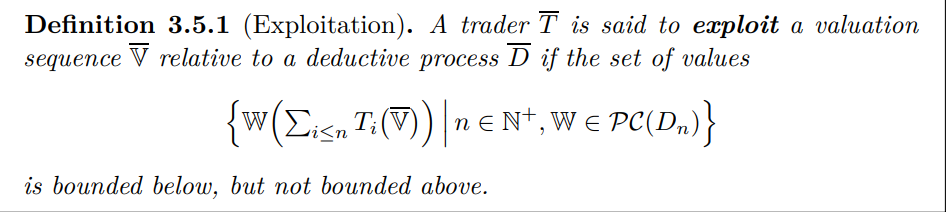
\includegraphics[width=1\linewidth]{image.png}
			    
			    \label{fig:placeholder}
			\end{figure}
			\item \textbf{Logical induction criterion:} No \textit{efficiently computable} (polytime) trader can exploit $\mathbb{P}$ relative to $D$
			\item Analogy: the classical Dutch book argument says ``no trader at all can exploit you $\Rightarrow$ your beliefs satisfy the probability axioms.'' Logical induction weakens this to ``no \textit{efficient} trader can exploit you,'' and this single condition implies a wide range of desirable properties
		\end{itemize}
		}
	\end{block}
	
}


	\frame{\frametitle{Logical Induction: Construction Sketch}
	\begin{block}{How to build a logical inductor}
		{\tiny
		\begin{itemize}
			\item Trading strategies are affine combinations of expressible features, so they can be \textit{aggregated}: any finite collection of traders can be summed into a single combined trader. In fact, an infinite sequence of traders can be combined (via a convergent weighted sum) into a single trader that exploits the market if \textit{any} of the individual traders do
			\item So it suffices to defend against a single combined trader $\overline{T}$ that represents all e.c.\ traders at once
			\item \textbf{Finding fair prices via fixed points.} On each day $n$, the algorithm looks at the combined trader's strategy $\overline{T}_n$ and the prices $\mathbb{P}_{\leq n-1}$ from previous days. It uses an approximate fixed point (guaranteed to exist by \textit{Brouwer's fixed point theorem}) to find prices $P_n$ such that the combined trader's profit $\overline{T}_n(\mathbb{P}_{\leq n})$ is at most a very small positive amount 
			\item Intuitively, the fixed point finds the trader's ``fair prices'' -- prices at which the trader on net abstains from betting, by adjusting prices upwards if the market buys more shares on net and vice versa
			\item Since the combined trader's profit on each day is bounded by a small $\epsilon_n$ with $\sum_n \epsilon_n < \infty$, cumulative profit is bounded, so no e.c.\ trader achieves unbounded profit -- the logical induction criterion is satisfied
		\end{itemize}
		}
	\end{block}
}
	
\frame{\frametitle{Logical Induction: Desirable Properties}
	\begin{block}{Properties of logical inductor}
		{\tiny
		\begin{itemize}
			\item \textbf{Convergence and Coherence:} In the limit, the prices of a logical inductor describe a belief state that is fully logically consistent -- $P_\infty(\varphi) \leq P_\infty(\psi)$ whenever $\varphi \Rightarrow \psi$, probability 1 to all theorems, 0 to all contradictions
			\item \textbf{Learning Statistical Patterns:} E.g.\ learns to assign $\approx 10\%$ to the claim ``the $n$th digit of $\pi$ is a 7'' for large $n$, even without computing those digits
			\item \textbf{Expectations:} Logical inductors give rise to a well-behaved notion of the expected value of a logically uncertain variable
			\item \textbf{Self-Trust:} A logical inductor's current credence in any sentence is a weighted average of its expected future credences -- it defers to its future self without needing to witness the reasoning trace of its future self
		\end{itemize}
		}
	\end{block}
}


\frame{\frametitle{Embedded Subproblem: Decision Theory}
	\begin{block}{The problem of counterfactuals for embedded agents}
		{\tiny
		\begin{itemize}
			\item For a dualistic agent (playing a video game), optimization is simple: just $\arg\max_a \mathbb{E}[U \mid \text{do}(A=a)]$ over actions
			\item For embedded agents, which action you pick is just another fact about the world. There is no well-defined notion of ``what would happen if I took a different action''
			\item Different decision theories correspond to different ways of constructing these counterfactuals: conditioning on the action as evidence (EDT), intervening causally on it (CDT), or reasoning about the logical consequences of being the kind of agent that runs a given decision procedure (FDT). 
		\end{itemize}
		}
	\end{block}
	
}
\frame{\frametitle{Causal decision theory}
	\begin{block}{Causal decision theory and the do-calculus}
		{\tiny
		\begin{itemize}
			\item A Bayesian network encodes conditional independences via a directed acyclic graph. The joint distribution factorizes as:
			$$P(X_1, \ldots, X_n) = \prod_{i=1}^{n} P(X_i \mid \text{Pa}(X_i))$$
			where $\text{Pa}(X_i)$ are the parents of $X_i$ in the graph
		\end{itemize}
		\begin{center}
			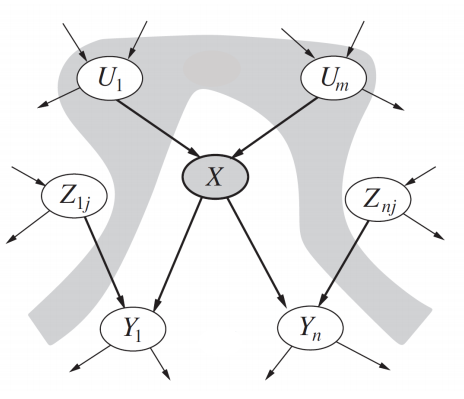
\includegraphics[width=0.17\linewidth]{bayesnet.png}
		\end{center}
		\begin{itemize}
			\item The $\text{do}$-operator models an intervention: $\text{do}(X = x)$ \textit{severs} all incoming arrows to $X$ (removing the influence of $X$'s parents) and fixes $X = x$, then propagates consequences downstream:
			$$P(Y \mid \text{do}(X = x)) = \sum_{u, z} P(Y \mid X{=}x, U{=}u, Z{=}z)\, P(U{=}u)\, P(Z{=}z)$$
			\item CDT chooses $a^* = \arg\max_a \mathbb{E}[U \mid \text{do}(A = a)]$: intervene on the action node and maximize expected utility under the resulting distribution
		\end{itemize}
		}
	\end{block}
	
}

\frame{\frametitle{Functional Decision Theory}
	\begin{block}{Twin Prisoner's Dilemma}
		{\tiny
		\begin{itemize}
			\item You and your psychological twin must each choose to cooperate or defect. You reason identically but choose in separate rooms without communication
			\item \textbf{CDT reasoning:} ``My action cannot causally affect my twin's action. No matter what she does, I gain extra by defecting. Defection dominates cooperation.'' Both defect.
			\item But your twin is computing the \textit{same decision function}. If your decision procedure outputs ``defect'', so does hers. The relevant question is not ``what should I do holding her action fixed?'' but ``what output of this decision procedure would yield the best outcome?''
		\end{itemize}
		}
	\end{block}
	\begin{block}{FDT: reasoning about the logical output of your decision procedure}
		{\tiny
		\begin{itemize}
			\item FDT asks: ``Which output of this very decision function I'm using would yield the best outcome, given everything in the world that depends on this function's output?''
			\item In the twin PD: if this function outputs cooperate, both copies would cooperate. If it outputs defect, both would defect. So FDT cooperates
			\item  FDT is sensitive to whether the correlation between your action and the world arises from a \textit{logical dependence}. It acts as if it controls both its own action and the action of its copy.
			\item FDT performs well in environments that contain copies of you, or predictors that model your decision procedure -- precisely the settings that arise for embedded agents
		\end{itemize}
		}
	\end{block}
}

\frame{\frametitle{Updateless Decision Theory}
	\begin{block}{Reflective stability of decision theories}
		{\tiny
		\begin{itemize}
			\item We want decision theories to be \textit{reflectively stable}: the decision theory shouldn't want to self-modify into a different decision theory
			\item CDT defects in the twin prisoner's dilemma, but \textit{before entering the game}, a CDT agent would pay to precommit to cooperating -- it would like to self-modify into an FDT agent. This means CDT is not reflectively stable
		\end{itemize}
		}
	\end{block}
	\begin{block}{From updateful to updateless}
		{\tiny
		\begin{itemize}
			\item \textbf{Updateful (EDT):} choose the action that maximizes expected utility \textit{given your current observations}:
			$$\texttt{choice}(o) := \arg\max_{a \in A}\; \mathbb{E}_P[U \mid \texttt{choice}(o) = a,\; O = o]$$
			\item \textbf{Updateless (UDT):} drop the conditioning on observations -- choose the action you would have wanted to commit to \textit{before} seeing anything:
			$$\texttt{choice}(o) := \arg\max_{a \in A}\; \mathbb{E}_P[U \mid \texttt{choice}(o) = a]$$
		\end{itemize}
		}
	\end{block}
	
}
\frame{\frametitle{Updateless Decision Theory}
\begin{block}{UDT as coordination across counterfactual branches}
		{\tiny
		\begin{itemize}
			\item \textbf{Blackmail:} giving in to blackmail achieves higher utility \textit{when you're being blackmailed}. But giving in incentivizes blackmail -- so an updateful agent conditions gives in to blackmail when it is being blackmailed.
			\item UDT asks: ``what \textit{policy} (mapping from observations to actions) would I have wanted to commit to before seeing any observations?'' Being the kind of agent that refuses blackmail is the better policy overall, even though it is locally costly when blackmailed
			\item  UDT agent coordinates across all counterfactual branches: by refusing to give in, the blackmailed branch sacrifices utility so that the branches where blackmail is never attempted becomes more probable. The overall policy maximizes expected utility across all branches, evaluated from the prior
			\item UDT is reflectively stable: a UDT agent would not want to self-modify into something else, because it is already following the policy it would have chosen to commit to from the start
		\end{itemize}
		}
	\end{block}
    }

\section{Descriptive Agent Foundations}
\frame{\frametitle{Descriptive Agent Foundations}
	\begin{block}{From normative to descriptive}
		{\tiny
		\begin{itemize}
			\item \textbf{Normative (ideal) agent foundations:} characterizes how a perfectly rational agent \textit{should} reason and act in principle -- starts from desiderata of ideal agents and derives what follows
			\item \textbf{Descriptive agent foundations:} asks what agents we actually encounter in the wild actually \textit{look like} -- given any physical system (a neural network, a bacterium, a future AI), can we identify its goals, world-model, and decision-making structure?
			\item The aim is to develop concepts that apply to a wide range of intelligences, from bacteria to superintelligences
		\end{itemize}
		}
	\end{block}
	\begin{block}{World-centric framing and robustness to scale}
		{\tiny
		\begin{itemize}
			\item Normative agency usually starts from the agent's subjective point of view (beliefs, preferences, rational choice). Embedded agency asks how this subjective picture maps onto a world where the agent is just another physical subsystem
			\item Descriptive agent foundations starts from the other direction: it begins with properties of the \textit{world} (e.g.\ modularity, selection pressures, resource constraints) and asks what sorts of processes reliably steer the world into narrow target configurations
			\item \textbf{Robustness to scaling up:} normative foundations demands that our concepts do not break when the agent becomes vastly more capable than us -- a safety property that fails under extreme optimization pressure is useless
			\item \textbf{Robustness to scaling down:} descriptive foundations additionally demands that the same framework degrades gracefully when applied to simpler systems.
		\end{itemize}
		}
	\end{block}
}
\frame{\frametitle{Descriptive Agent Foundations}
	\begin{block}{Physical constraints shape agent structure}
		{\tiny
		\begin{itemize}
			\item Descriptive foundations emphasize selection pressures, constraints from the physical world, and computational boundedness -- these determine what kinds of agents actually arise
			\item  For instance, a key property of the world is \textbf{modularity}: the world decomposes into subsystems that interact sparsely. This should make both planning and world-modelling easier for any agent that exploits it
			\item \textbf{World-modelling:} Bayesian networks exploit modularity -- instead of maintaining a full joint hypothesis over every possible world, updates about variables are only propagated locally along edges in the graph
			\item \textbf{Planning:} General-purpose search exploits modularity -- if the world is modular, an agent can pursue decoupled subgoals independently, rather than having to plan everything jointly
		\end{itemize}
		}
	\end{block}
}

\frame{\frametitle{Optimization and Thermodynamics}
	\begin{block}{Optimization as local entropy reduction}
		{\tiny
		\begin{itemize}
			\item Powerful agents reliably steer the world towards narrow regions of target configurations -- outcomes that would be extremely unlikely to arise under any random process
			\item This is a form of \textit{local entropy reduction}: concentrating probability mass from a broad initial distribution onto a narrow final distribution around a target
			\item Irreversible transitions: funnelling many initial states into the same targets
			\item Existing results in stochastic thermodynamics such as fluctuation theorems (Second law of thermodynamics), cost of information erasure and information thermodynamics directly constrains the shape of optimization processes and hold far from equilibrium
		\end{itemize}
		}
	\end{block}
}


\frame{\frametitle{Optimization  and Thermodynamics}
	\begin{block}{Steering costs information (Touchette \& Lloyd)}
		{\tiny
		\begin{center}
			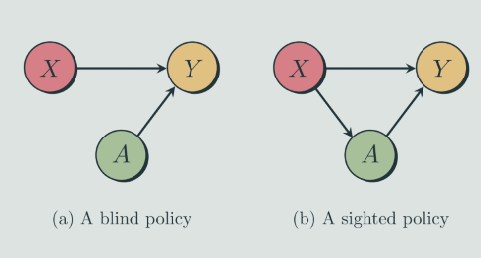
\includegraphics[width=0.45\linewidth]{lloyd.png}
		\end{center}
		\begin{itemize}
			\item A \textit{sighted} agent observes $X$ and chooses action $A$ accordingly; a \textit{blind} agent acts independently of $X$. The entropy reduction a sighted agent can achieve over the blind baseline is bounded:
			$$\Delta H \leq \Delta H_{\text{Blind}}^{\text{Max}} + I(X; A)$$
			\item The degree to which an agent can steer outcomes beyond what a blind policy achieves is paid for by the mutual information between its observations and its actions -- optimization requires information
		\end{itemize}
		}
	\end{block}
}

\frame{\frametitle{Optimization  and Thermodynamics}
	\begin{block}{From ensembles to individual states}
		{\tiny
		\begin{itemize}
			\item Traditional thermodynamics defines entropy in terms of probability distributions over ensembles -- but where does the distribution come from?
			\item \textbf{Algorithmic thermodynamics} (Ebtekar \& Hutter) replaces Shannon entropy $H$ with Kolmogorov complexity $K$, yielding thermodynamic laws that apply to \textit{individual physical states} rather than ensembles
            \item Intuitively, a state in which all particles are concentrated in one location would have low entropy, because the repeated coordinates can be printed by a short program.
		\end{itemize}
		}
	\end{block}
	\begin{block}{Knowledge as an endogenous physical resource}
		{\tiny
		\begin{itemize}
			\item In the Gibbs-Shannon framework, a probability distribution $\mu$ is an \textit{exogenous} parameter specifying what the agent knows. But the insight from embedded agency is that an embedded agent's knowledge must be \textit{physically encoded} in its brain or memory device
			\item In algorithmic thermodynamics, knowledge becomes an \textit{endogenous} feature of the physical system: it manifests as \textbf{algorithmic mutual information} between the agent's memory and the environment
			\item This algorithmic mutual information plays same role as the setting in Touchette \& Lloyd: it is the resource that an embedded agent can spend to steer the world into narrow target configurations
			\item From the embedded perspective: the agent's probabilistic knowledge about the environment is physically encoded in its memory, and this manifests as algorithmic mutual information between agent and environment. This algorithmic mutual information is precisely the resource that can be spent on steering -- which is why an agent that \textit{knows more} about its environment can perform \textit{more optimization}
		\end{itemize}
		}
	\end{block}
}


\frame{\frametitle{Conclusion}
	\begin{block}{Conclusion}
		{\tiny
		\begin{itemize}
			\item We need robust concepts about agency to reason about systems far more capable than anything we have seen, and we need properties that are invariant under self-modification. 
			\item \textbf{Tiling agents:} directly about making safety a reflectively stable property -- ensuring that an agent's successors preserve the same guarantees, indefinitely
			\item \textbf{Logical induction:} about reasoning under logical uncertainty in an environment larger than yourself, where you cannot instantly compute the consequences of your hypotheses. Also relevant for reasoning about your own future beliefs and inputs -- a form of self-reference
			\item \textbf{Decision theory:} a reflectively consistent degree of freedom -- an agent using a bad decision theory will not automatically self-correct as it gets smarter. Also directly tied to embedded agency: counterfactuals are not well-defined when you are part of the environment, and the environment may contain copies of you or predictors modelling your decision procedure
			\item \textbf{Descriptive agent foundations:} starts from properties of the world (modularity, selection pressures, thermodynamic constraints) and derives what kinds of optimization processes arise -- what agents embedded in the physical world would look like mechanistically
			\item \textbf{Connecting the two viewpoints:} reasoning about how properties of the world constrain the structure of optimization processes may tell us how an ideal agent \textit{should} model the world and plan its actions from its subjective point of view
		\end{itemize}
		}
	\end{block}
}


\end{document}